\subsection{Cenário típico}
    \par Para se ter um entendimento antes da aplicação da Arquitetura Limpa, na segunda etapa do presente trabalho de maneira prática, principalmente em relação a estrutura de pastas e organização geral do projeto de software e comunicação dos componentes, deve-se inicialmente analisar a obra de \cite{livro:martin:cleanarch} em relação ao que ele propõe como modelo de organização e fluxo de informações na Arquitetura Limpa.

    \par Tendo isso em vista, nota-se o uso do termo "Arquitetura Gritante", tal termo é referente a um conceito proposto e defendido pelo autor, que prega que a estrutura de um sistema de software deve, antes de qualquer coisa, comunicar o seu propósito e seus casos de uso. Sendo assim a arquitetura de uma aplicação deve revelar de maneira clara, o seu domínio de negócio, como por exemplo, "Sistema de segurança de trabalho", "Sistema de gestão para o terceiro setor". Assim Indo contra a ideia de que a arquitetura deve ser definida pelo seu framework, como Rails ou Spring, pois são referentes a ferramentas e não ao objetivo do software \cite{livro:martin:cleanarch}.

    \par Portanto, o principal objetivo de uma Arquitetura Gritante é ser centrada nos casos de uso e desacoplá-los de detalhes de implementação, desse modo a estrutura passa a ser o reflexo do software em si, permitindo uma melhor compreensão da sua finalidade de negócio, antes mesmo de se conhecer a infraestrutura tecnológica \cite{livro:martin:cleanarch}.

    \par Com o conceito de Arquitetura Gritante explicado e para o melhor entendimento da abordagem proposta por \cite{livro:martin:cleanarch} em relação a organização e o fluxo das informações na Arquitetura Limpa, pode-se analisar o que o autor define em seu livro como um \textbf{cenário típico} de implementação da Arquitetura Limpa, tal cenário representa uma aplicação Java WEB, tais conceitos podem ser implementados em outras linguagens de programação orientadas à objetos, o que torna essa análise útil para o objetivo deste trabalho.

    \begin{figure}[H]
        \centering
        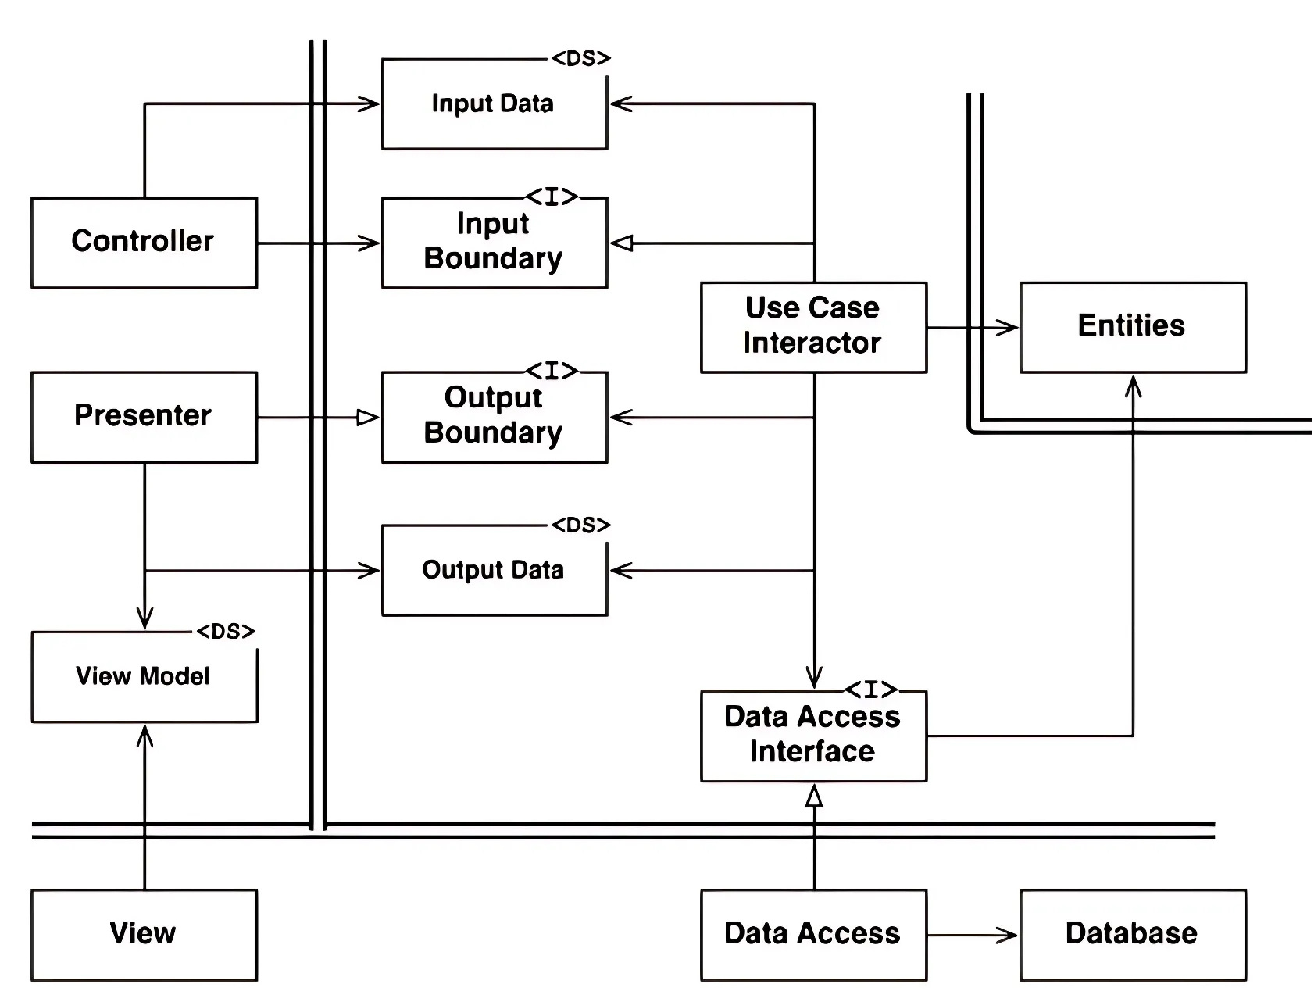
\includegraphics[width=1\linewidth]{figuras/clean_arch/typical_scenario.pdf}
        \caption{Um cenário típico para um sistema Java baseado em web utilizando uma base de dados.}
        \label{fig:typical_scenario} 
        \newcommand{\minhafonte}{Fonte: \cite{livro:martin:cleanarch}.}
        \minhafonte
    \end{figure}

    \par Nota-se na Figura \ref{fig:typical_scenario} a representação feita por \cite{livro:martin:cleanarch} representando esse cenário, onde, o fluxo de dados é controlado pelos seguintes componentes:

    \begin{itemize}
        \item \textbf{Controller:} É o ponto de entrada da aplicação, ele recebe a requisição do mundo externo. Sua função é desempacotar os dados vindos da requisição, agrupá-los em uma estrutura de dados simples e indiferente em relação a frameworks e passar esses dados para o interior da arquitetura através da \textbf{InputBoundary}.

        \item \textbf{InputBoundary:} É uma interface pertencente à camada de Casos de Uso da arquitetura limpa. Ela representa o \textbf{UseCaseInteractor}, o Controller depende e invoca esta interface para transmitir os dados. Ela serve como uma porta de entrada que isola o núcleo de negócio do mecanismo de entrega e garante que a dependência aponte para dentro, em conformidade com a Regra da Dependência.

        \item \textbf{UseCaseInteractor:} Este componente implementa a interface \textbf{InputBoundary}. Ele contém a regra de negócio específica da aplicação, recebe o objeto de dados simples e orquestra a interação com as Entities para executar a funcionalidade. Para a saída, ele não chama o Presenter diretamente, mas sim a interface \textbf{OutputBoundary}.


        \item \textbf{Entities:} São objetos que encapsulam as regras de negócio mais gerais e de mais alto nível do software. Elas são manipuladas pelo \textbf{UseCaseInteractor}, mas não possuem conhecimento sobre ele ou qualquer outra camada externa, garantindo sua total independência.
        
        
        \item \textbf{DataAccessInterface:} É uma interface definida na camada de Casos de Uso da Arquitetura Limpa, que especifica os métodos de persistência necessários, como buscar ou salvar \textbf{Entities}. Essa abordagem, desacopla o caso de uso da implementação real do BD.
        
        \item \textbf{OutputBoundary:} Parecida com a \textbf{InputBoundary}, esta é uma interface definida na camada de Casos de Uso. Sendo ela a representação do Presenteer, o \textbf{UseCaseInteractor} utiliza ela para enviar os dados de resultado para fora, sem conhecer a existência ou a natureza do \textbf{Presenter}, tal técnica completa o mecanismo de inversão de dependência.
        
        \item \textbf{Presenter:} É a implementação da interface \textbf{OutputBoundary}. Sua responsabilidade é receber os dados de negócio crus do caso de uso e formatá-los para exibição, convertendo os dados em uma estrutura chamada \textbf{View Model}.
        
        
        \item \textbf{ViewModel:} É a estrutura de dados mais simples que contém apenas strings, booleanos ou outros tipos de dados prontos para serem exibidos na \textbf{View}, tal estrutura de dados não tem nenhuma lógica de negócios.
        
        
        \item \textbf{View}: É o último componente no fluxo e é responsável por exibir os dados na tela para o usuário, ou caso seja uma API, exibir o JSON ou outro formato definido na \textbf{ViewModel}.

    \end{itemize}
